\jxhj{%教学后记
	}
\skrq{%授课日期
	2017年10月31日 4-5节}
\ktmq{%课题名称
	 外轮廓加工}
\jxmb{%教学目标,每行前面要加 \item
	\item 掌握增加刀路去残料的思路;
	\item 掌握增加刀路的方法;
	\item 掌握相关点的计算;
	\item 会合理的增加刀路	。 }
\jxzd{%教学重点,每行前面要加 \item
	\item 增加刀路去残料的思路;
	\item 增加刀路的方法。 }
\jxnd{%教学难点,每行前面要加 \item
	\item 相关点的计算。 }
\jjff{%教学方法
	通过讲述、举例、演示法来说明;}

\makeshouye %制作教案首页

%%%%教学内容
\subsection{组织教学}
\begin{enumerate}[\hspace{2em}1、]
	\item 集中学生注意力;
	\item 清查学生人数;
	\item 维持课堂纪律;
\end{enumerate}

\subsection{复习导入及主要内容}
\begin{enumerate}[1、]
\item 平面的加工工工艺;
\item 斜面的加工工艺;
\item 形位公差;
\item 编程实例。
\end{enumerate}

\subsection{教学内容及过程}
\subsubsection{加工实例}
在数控机床上加工如图\ref{fig:14-1}所示的零件,试完成加工工艺的分析与加工程序的编写,并完加成零件的加工。

\begin{figure}[h]
	\centering
	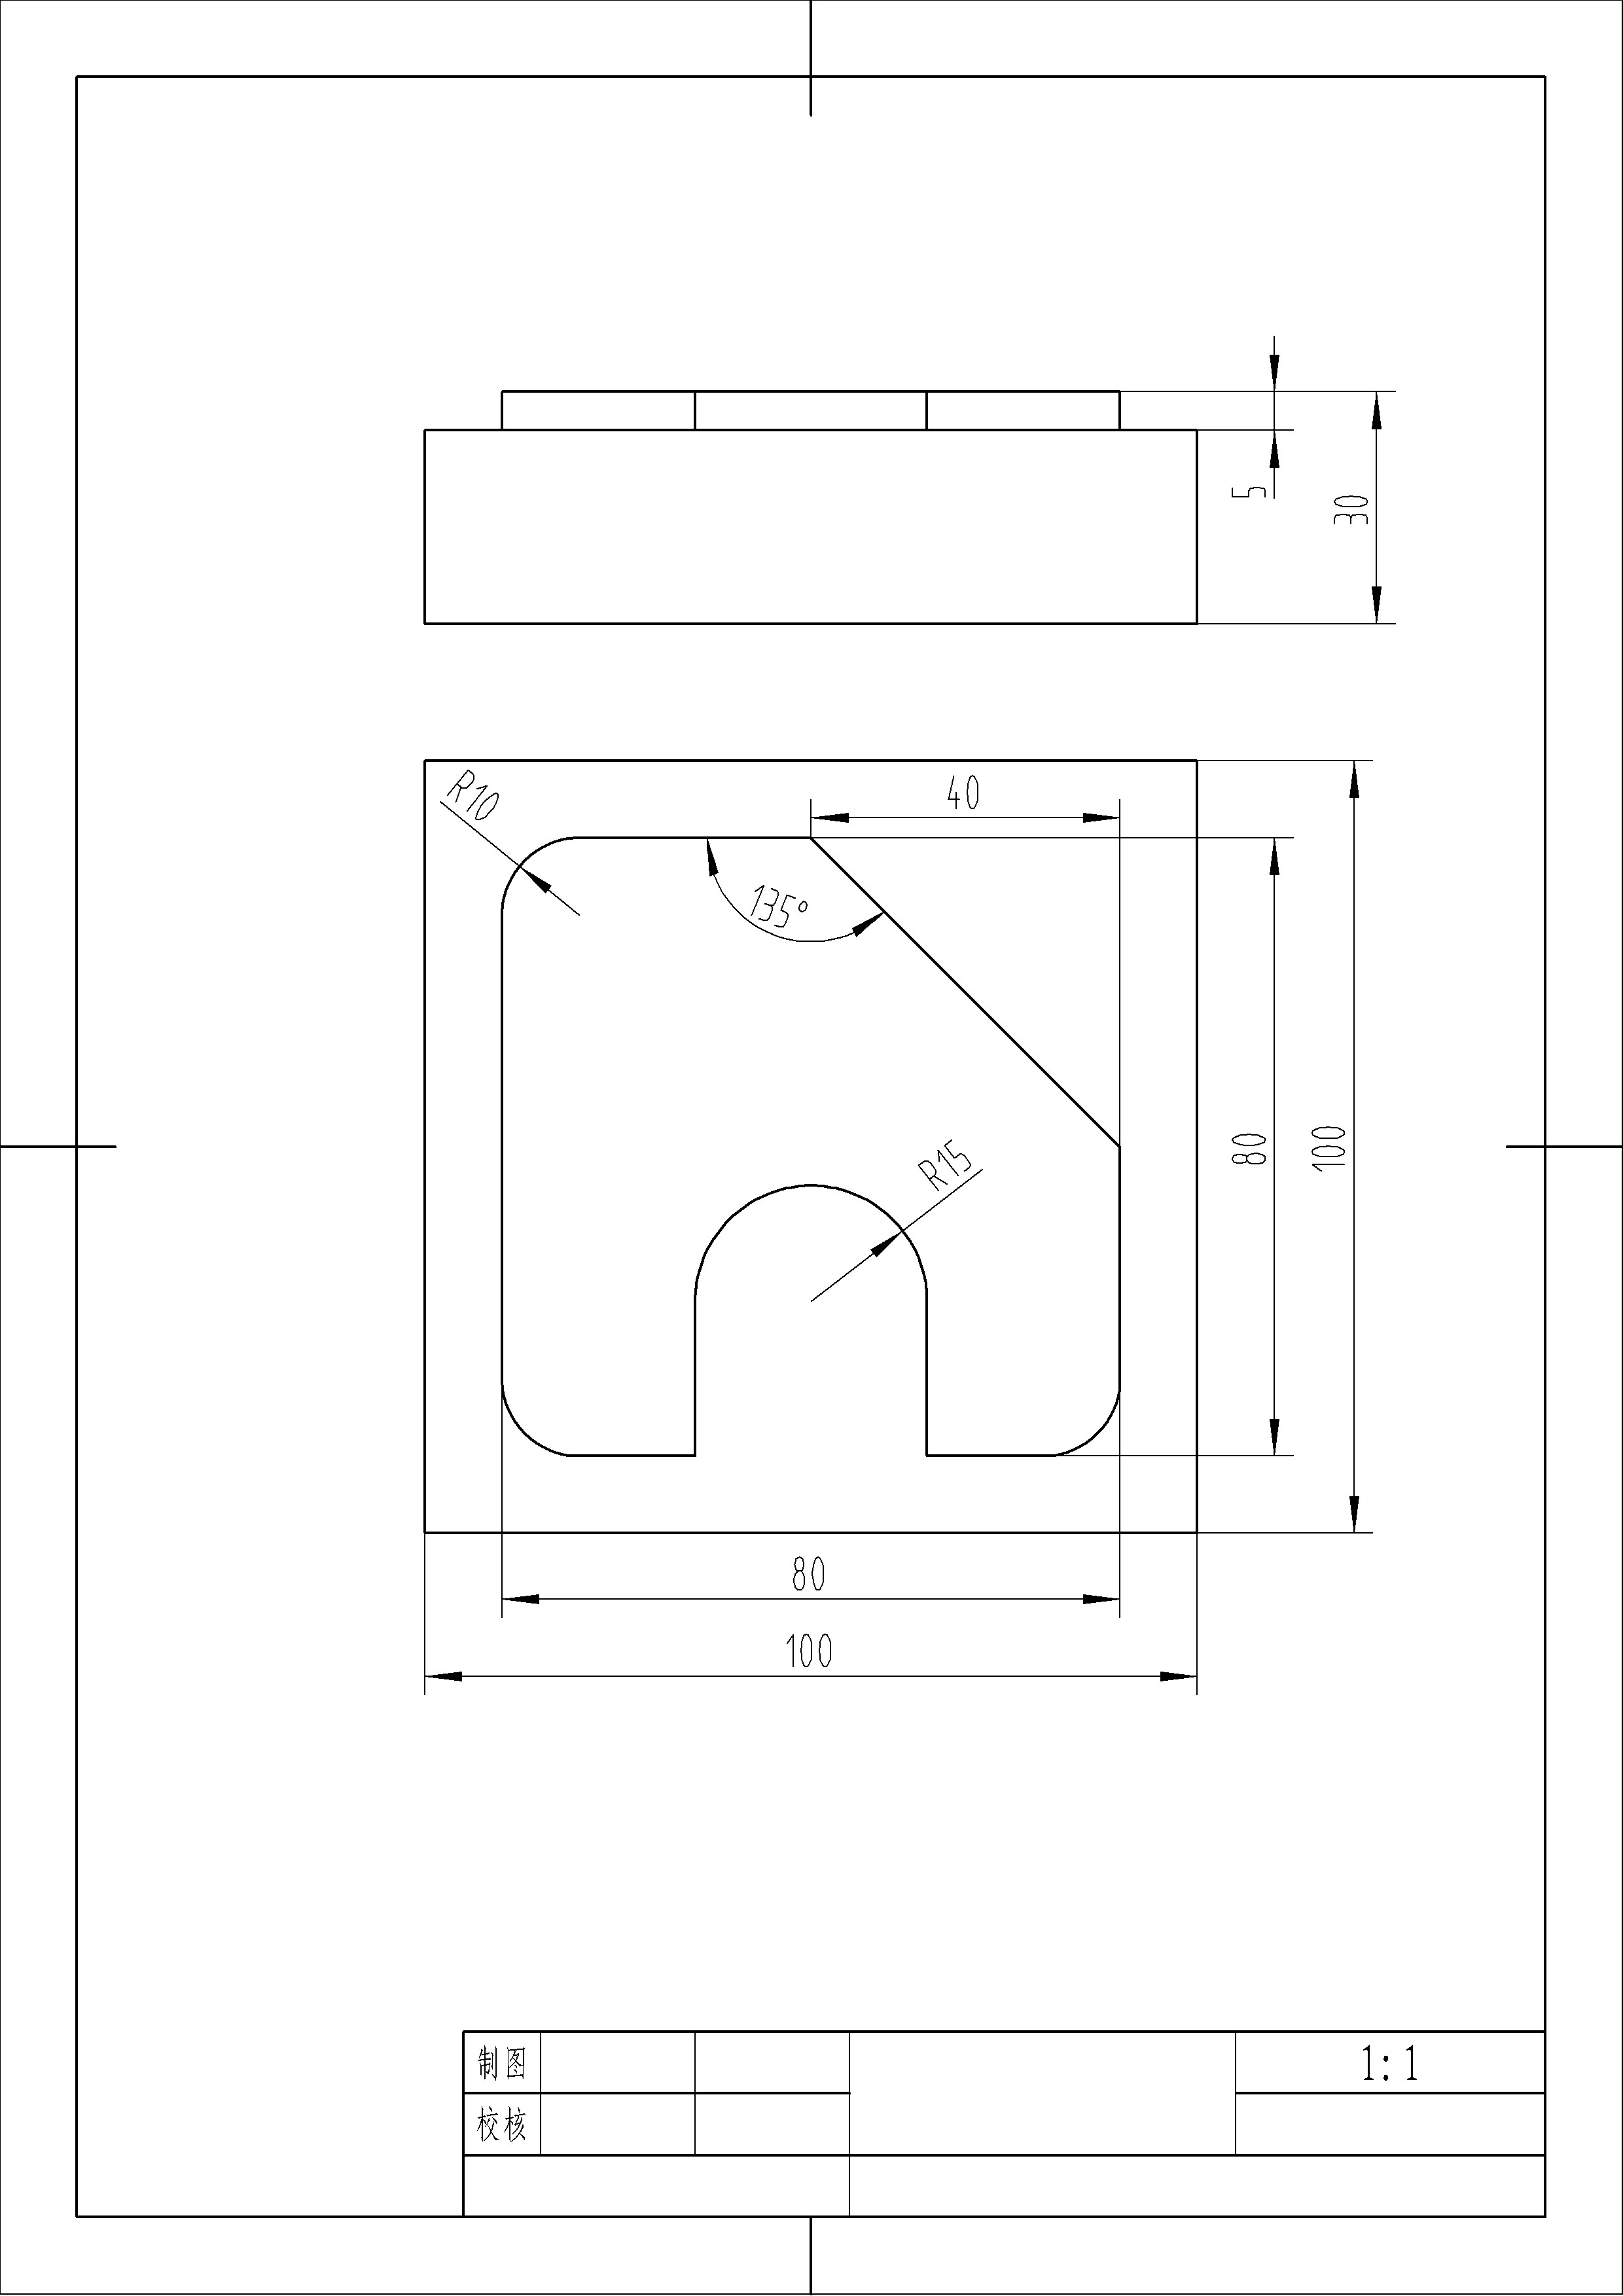
\includegraphics[width=0.8\linewidth,trim=130 200 80  120,clip]{data/image/14-1.jpg}
	\caption{刀补实例}
	\label{fig:14-1}
\end{figure}

1、残料计算:

三个角处的残料为 $20\sqrt{2}-10=18.28$

大角处的残料为  $50\sqrt{2}-20\sqrt{2}=30\sqrt{2}=42.42$

则无论用多大的刀具,此处的残料都不能用刀具半径补偿功能进行去残料。

2、增加刀路去残料:

适合所有类型的去残料,

难点:刀路怎么设计,相关点的计算

基本要求:不能过切,粗加工后能把所有残料去完

自动编程软件:自动计算:

平行往复走刀

沿部件平行环切

沿毛坯平行环切

螺旋高速切削

手工编程:选计算较简单的方法

常用去残料刀路设计:


角

大圆

3、刀路设计:

刀具:铣平面及粗加工:\diameter 12立铣刀

加工宽度10mm

精加工\diameter 10立铣刀

去残料刀路:

角点坐标:

R10--R16.5(粗加工)--R26.5($18.5-16.5=2$)残料去完--改成直线(切线)

$20\sqrt{2}-26.5=2.32$

两边的长:$2.32\sqrt{2} =3.28$

点A(50,-46.)  B(46,-50)

其余根据对称点进行计算

G1 X50. Y-46. 

X46. Y-50.

中间下面的半圆槽:

直线:$C(0,-60) D(0,-20)$


大角:   

$28.28+6.5$ (粗加工) 

$28.28+16.5=44.78$(相当于刀补16.5)

坐标 $ X=50-(70.7-44.78)\sqrt{2} 
=13.349$

$28.28+26.5=54.78 $(相当于刀补26.5)

$X=50-(70.7-54.78)\sqrt{2} 
=27.489$

$28.28+36.6=64.78$(相当于刀补36.5)$+6=42.5$去完

$X=50-(70.7-64.78) \sqrt{2}
=41.629$

G1 X50 Y50

X41.629

X50 Y41.629

Y27.489

X27.489Y50

X13.349

X50 Y13.349

4、程序编写
\begin{lstlisting}

O1(粗加工主程序)
G54G17G40G49G90
M3S500
G1Z20.F2000
X70.Y70.
Z3.0
Z-5. F200
M98P2(去残料)
Z5.0
X0Y60.
Z-5.0
D1M98P3
G1Z30.F2000
M5 
M30
\end{lstlisting}

\begin{lstlisting}
O2(去残料子程序)
N1 G1 X50 Y50
X41.629
X50 Y41.629
Y27.489
X27.489Y50
X13.349
X50 Y13.349
X60.
N2 Y-46.
X50.
X46.Y-50.
Y-60
N3X-46.
Y-50.
X-50.Y-46.
Y-60.
N4 Y46.
X-50
X-46.Y50.
Y60.
M99;
\end{lstlisting}

\begin{lstlisting}
O3(轮廓子程序)
G1X-10.Y50.
G3X0Y40.R10.
G1X40.Y0
G1Y-30.
...

...

\end{lstlisting}












\begin{lstlisting}
O4(精加工主程序)
G54G17G40G49G90
M3S800
G1Z20.F2000
X0.Y60.
Z3.0
Z-5. F200
Z-5.0
D1M98P3
G1Z30.F2000
M5 
M30
\end{lstlisting}




\subsection{课堂小结}
\begin{enumerate}[1、]
	\item 增加刀路去残料;
	\item 加工实例;
	\item 相关计算。
\end{enumerate}

\vfill
\subsection{布置作业}
\begin{enumerate}[1、]
	\item 编写上面的程序。
\end{enumerate}
\vfill